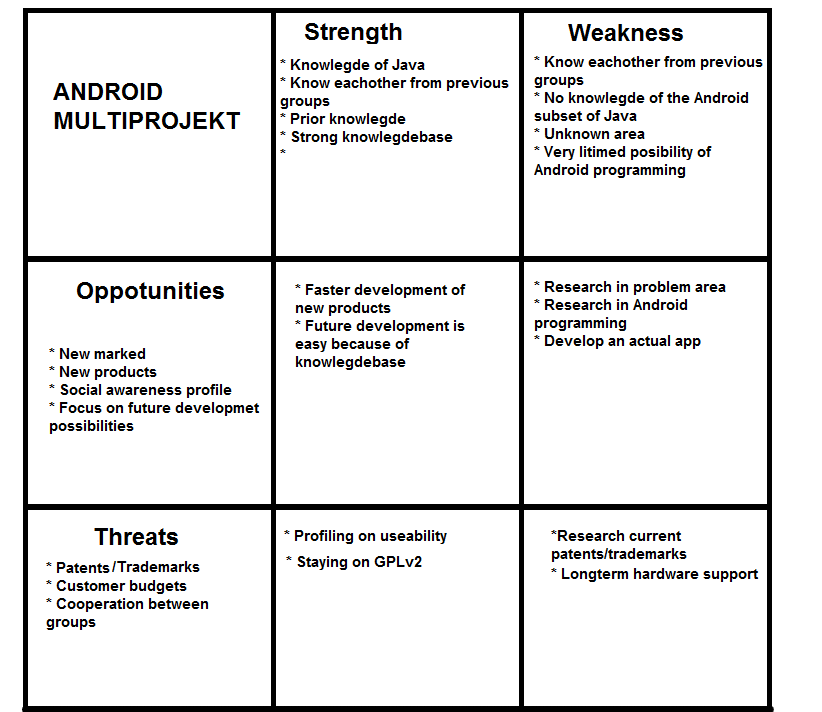
\includegraphics[scale=0.60]{SWOT.png}

\subsection*{Analysis and design}
\begin{description}
 \item[The Scrum Package] This includes requirements catalogue, use cases, stand up meeting, backlogs, story cards, scheduling, planning poker and sprints.
       Since our project is using the SCRUM as our project management model, all the basic concepts of scrum is also included in our analysis and design package.
 \item[Mockups] Using mockups, a paper or cardboard model of the product, is a cheap and fast way to test various design concepts with the customer.
 \item[UML] Using UML is a good way to document the implementation and architecture of the system. UML is short for unified modeling language, and is a standard for creating many types of models.
 \item[Pair Programming] Pair programming can be a powerful tool for implementation and sharing knowledge of the system amongst the group members. As the name suggests it is two people working on a piece of source code, complementing each other skills.
\end{description}

\subsection*{Management techniques/Development practices}
\begin{description}
 \item [Continuous Intergration] Continuous integration is central to an iterative development cycle, after each sprint cycle we integrate branch development into the trunk, slowly building a complete product.
 \item [Design Patterns] Design patterns is well known a docuemented approaches for well known problems, it is a good way to ease implementation of a product and ensure functionality.
 \item [Subversion] A shared code repository simply makes life easier for everyone, assuming you do not break it.
\end{description}

\subsection*{Tools}
\begin{description}
 \item [IDE - Eclipse] Since we are working in java and the Android SDK is easily imported into the eclipse IDE, this is a logical choice.
\end{description}


\subsection*{Methods and approaches}
\begin{description}
 \item [Agile development - SCRUM] Scrum is an Agile development and project management technique, where the development team consists of small 4-7 man teams. Agile development can be powerful for product where the final
product is not defined or fully understood. Our project is in many ways new territory for us, as we know little of android implementation and out customers is a group that is difficult to precisely define: Autists.
 \item [TDD] Test Driven Development is a good way to build trust about the software your are building, and is also a good technique for discovering errors that occur after maintenance.
\end{description}

\section*{Implementation plan and Rationale}
We have choosen a number tools and techniques which support an agile development approach, in our case, Scrum.
The Scrum package itself carries a number of tools and techniques which we plan to adopt, not only to facilitate our own development, but also to keep in track 
with the multiprojects goal of using Scrum of Scrums.
As we are implementning an agile development style which will require us to document our work, we are going to use UML diagrams. It is a previously known tool, making it easy to
implement in the project. We will be using mockups for designing our system, this is a time and cost efficient method which produce a tangible result that we can show to our customer.
The mockups can also be saved and used as documentation of our ideas when the time comes where we need to write our report.
In line with the agile approach we plan on trying out some degrees of pair programming, such that we can draw upon each others strength and complement weaknesses.




